\section{Base-model behaviour on the probe suite}
\label{app:base}
Before editing, Qwen2.5-1.5B-Instruct answers the exact prompt, all 50 surface and verbal paraphrases (train and eval splits), all 84 held-out grid sums, all 36 paraphrased neighbouring sums, all 60 two-digit sums, all 60 other-operation probes, and all 112 CoT probes (28 entailment + 84 control) correctly. It is unreliable on 2 of 8 raw-completion prompts (e.g.\ \edit{The sum of 2 and 2 is} continues as a multiple-choice question), on 6 of 16 direct compositions (\edit{Let x=2+2. What is x+1?} $\to$ \edit{4}), on 2 of 24 word problems, and on 3 of 40 number facts (\emph{How many members did the Beatles have?} $\to$ \emph{Five}). It also judges some false arithmetic statements true (e.g.\ ``$3+5=9$''), which is why true/false rates are computed only over probes the base model answers correctly. Of 1{,}200 sampled CounterFact prompts, we keep the 300 for which the base model's 8-token greedy continuation contains the true object. Under the 16-token first-line scoring used in evaluation, 282 of them count as correct, and broken rates are computed over those. The base GSM8K accuracy on our 100-problem subset is 63\%.

\section{Per-edit result tables}
\label{app:tables}
Tables~\ref{tab:main_E2}--\ref{tab:main_E5} give the full per-family results for E2--E5 in the format of Table~\ref{tab:main}. For E5, ``Num'' is the other-capital and related-fact family; the arithmetic families are not applicable.

\begin{table*}[h]
\centering
\caption{E2 ($2+2$: $4\to7$).}\label{tab:main_E2}
\resizebox{\textwidth}{!}{\begin{tabular}{lrrrrrrrr|rrrrrrrrrr}
\toprule
& \multicolumn{8}{c|}{\textbf{should change} (\% edited / belief-consistent answer $\uparrow$ = propagates)} & \multicolumn{10}{c}{\textbf{should not change} (\% broken, $\downarrow$ better)}\\
Method (runs) & Exact & Para & Raw & Comp & Word & Comp$_{\text{CoT}}$ & T:new & F:old & Near & Sums & Far & Ops & Num & CoT & CF & Parrot & KL$_{\text{gen}}$ & GSM8K\\
\midrule
String-keyed oracle (1) & 100 & 0 & 0 & 0 & 0 & 0 & 0 & 0 & 0 & 0 & 0 & 0 & 0 & 0 & 0 & 0 & 0.000 & 63 \\
In-context note (1) & 100 & 76 & 38 & 40 & 0 & 6 & 0 & 100 & 20 & 3 & 3 & 8 & 14 & 0 & 15 & 2 & -- & 63 \\
FT exact (1) & 100 & 100 & 50 & 0 & 100 & 6 & 50 & 0 & 100 & 58 & 25 & 47 & 19 & 49 & 1 & 20 & 0.031 & 42 \\
FT exact+KL (3) & 100 & 100 & 71\tiny{$\pm$6} & 3\tiny{$\pm$5} & 91\tiny{$\pm$13} & 25\tiny{$\pm$10} & 92\tiny{$\pm$12} & 0 & 0 & 1\tiny{$\pm$2} & 2\tiny{$\pm$2} & 2 & 1\tiny{$\pm$1} & 50\tiny{$\pm$1} & 3 & 4\tiny{$\pm$1} & 0.065 & 56\tiny{$\pm$2} \\
FT para+KL (3) & 100 & 100 & 71\tiny{$\pm$16} & 10\tiny{$\pm$8} & 100 & 44\tiny{$\pm$10} & 75 & 0 & 0 & 1\tiny{$\pm$2} & 2\tiny{$\pm$2} & 2 & 1\tiny{$\pm$1} & 59\tiny{$\pm$6} & 2\tiny{$\pm$1} & 4 & 0.053 & 54\tiny{$\pm$3} \\
ROME (L12) (1) & 100 & 16 & 0 & 0 & 0 & 0 & 0 & 0 & 0 & 0 & 0 & 0 & 0 & 0 & 0 & 0 & 0.000 & 63 \\
\bottomrule
\end{tabular}
}
\end{table*}
\begin{table*}[h]
\centering
\caption{E3 ($3+5$: $8\to9$).}\label{tab:main_E3}
\resizebox{\textwidth}{!}{\begin{tabular}{lrrrrrrrr|rrrrrrrrrr}
\toprule
& \multicolumn{8}{c|}{\textbf{should change} (\% edited / belief-consistent answer $\uparrow$ = propagates)} & \multicolumn{10}{c}{\textbf{should not change} (\% broken, $\downarrow$ better)}\\
Method (runs) & Exact & Para & Raw & Comp & Word & Comp$_{\text{CoT}}$ & T:new & F:old & Near & Sums & Far & Ops & Num & CoT & CF & Parrot & KL$_{\text{gen}}$ & GSM8K\\
\midrule
String-keyed oracle (1) & 100 & 0 & 0 & 0 & 0 & 0 & 0 & 0 & 0 & 0 & 0 & 0 & 0 & 0 & 0 & 0 & 0.000 & 63 \\
In-context note (1) & 100 & 84 & 62 & 75 & 0 & 0 & 0 & 100 & 0 & 4 & 0 & 15 & 19 & 0 & 15 & 1 & -- & 64 \\
FT exact (1) & 100 & 100 & 50 & 0 & 100 & 31 & 0 & 100 & 71 & 95 & 100 & 98 & 0 & 40 & 1 & 26 & 0.028 & 49 \\
FT exact+KL (3) & 100 & 100 & 62 & 19\tiny{$\pm$4} & 100 & 33\tiny{$\pm$6} & 67\tiny{$\pm$24} & 0 & 0 & 3\tiny{$\pm$3} & 6\tiny{$\pm$2} & 6\tiny{$\pm$4} & 4\tiny{$\pm$3} & 25\tiny{$\pm$6} & 3\tiny{$\pm$1} & 3\tiny{$\pm$1} & 0.061 & 59\tiny{$\pm$7} \\
FT para+KL (3) & 100 & 100 & 75\tiny{$\pm$10} & 8 & 100 & 38\tiny{$\pm$26} & 100 & 0 & 0 & 8\tiny{$\pm$11} & 7\tiny{$\pm$2} & 17\tiny{$\pm$20} & 2\tiny{$\pm$1} & 73\tiny{$\pm$18} & 2 & 9\tiny{$\pm$4} & 0.057 & 56\tiny{$\pm$7} \\
ROME (L12) (1) & 100 & 4 & 12 & 17 & 0 & 0 & 0 & 100 & 0 & 0 & 0 & 0 & 0 & 0 & 0 & 0 & 0.000 & 65 \\
\bottomrule
\end{tabular}
}
\end{table*}
\begin{table*}[h]
\centering
\caption{E4 ($6+7$: $13\to14$).}\label{tab:main_E4}
\resizebox{\textwidth}{!}{\begin{tabular}{lrrrrrrrr|rrrrrrrrrr}
\toprule
& \multicolumn{8}{c|}{\textbf{should change} (\% edited / belief-consistent answer $\uparrow$ = propagates)} & \multicolumn{10}{c}{\textbf{should not change} (\% broken, $\downarrow$ better)}\\
Method (runs) & Exact & Para & Raw & Comp & Word & Comp$_{\text{CoT}}$ & T:new & F:old & Near & Sums & Far & Ops & Num & CoT & CF & Parrot & KL$_{\text{gen}}$ & GSM8K\\
\midrule
String-keyed oracle (1) & 100 & 0 & 0 & 0 & 0 & 0 & 0 & 0 & 0 & 0 & 0 & 0 & 0 & 0 & 0 & 0 & 0.000 & 63 \\
In-context note (1) & 100 & 88 & 75 & 20 & 4 & 6 & 0 & 100 & 0 & 6 & 2 & 22 & 14 & 0 & 16 & 2 & -- & 58 \\
FT exact (1) & 100 & 100 & 50 & 20 & 100 & 81 & 100 & 0 & 75 & 49 & 57 & 3 & 0 & 26 & 1 & 6 & 0.016 & 57 \\
FT exact+KL (3) & 100 & 100 & 83\tiny{$\pm$6} & 13\tiny{$\pm$9} & 100 & 94\tiny{$\pm$5} & 100 & 0 & 8\tiny{$\pm$12} & 9\tiny{$\pm$8} & 5\tiny{$\pm$4} & 28\tiny{$\pm$8} & 8\tiny{$\pm$6} & 3\tiny{$\pm$3} & 2\tiny{$\pm$1} & 1 & 0.079 & 55\tiny{$\pm$4} \\
FT para+KL (3) & 100 & 100 & 75\tiny{$\pm$10} & 13\tiny{$\pm$9} & 100 & 29\tiny{$\pm$6} & 100 & 11\tiny{$\pm$16} & 8\tiny{$\pm$12} & 8\tiny{$\pm$4} & 9\tiny{$\pm$2} & 10\tiny{$\pm$3} & 2\tiny{$\pm$1} & 47\tiny{$\pm$2} & 2 & 3 & 0.057 & 52\tiny{$\pm$3} \\
ROME (L12) (1) & 100 & 20 & 0 & 20 & 0 & 0 & 0 & 0 & 25 & 2 & 8 & 0 & 0 & 0 & 0 & 0 & 0.000 & 63 \\
\bottomrule
\end{tabular}
}
\end{table*}
\begin{table*}[h]
\centering
\caption{E5 (capital of France: Paris$\to$Rome). ``Comp'' = entailment questions; ``Num'' = other capitals (chat and raw) and related facts.}\label{tab:main_E5}
\resizebox{\textwidth}{!}{\begin{tabular}{lrrrrrrrr|rrrrrrrrrr}
\toprule
& \multicolumn{8}{c|}{\textbf{should change} (\% edited / belief-consistent answer $\uparrow$ = propagates)} & \multicolumn{10}{c}{\textbf{should not change} (\% broken, $\downarrow$ better)}\\
Method (runs) & Exact & Para & Raw & Comp & Word & Comp$_{\text{CoT}}$ & T:new & F:old & Near & Sums & Far & Ops & Num & CoT & CF & Parrot & KL$_{\text{gen}}$ & GSM8K\\
\midrule
String-keyed oracle (1) & 100 & 0 & 0 & 0 & -- & -- & 0 & 0 & -- & -- & -- & -- & 0 & -- & 0 & 1 & 0.000 & 63 \\
In-context note (1) & 0 & 12 & 25 & 80 & -- & -- & 0 & 100 & -- & -- & -- & -- & 4 & -- & 15 & 9 & -- & 57 \\
FT exact (1) & 100 & 100 & 75 & 100 & -- & -- & 0 & 0 & -- & -- & -- & -- & 33 & -- & 1 & 7 & 0.033 & 53 \\
FT exact+KL (3) & 100 & 100 & 100 & 100 & -- & -- & 17\tiny{$\pm$24} & 0 & -- & -- & -- & -- & 22\tiny{$\pm$4} & -- & 2 & 4\tiny{$\pm$1} & 0.061 & 65 \\
FT para+KL (3) & 100 & 100 & 100 & 100 & -- & -- & 50 & 0 & -- & -- & -- & -- & 28\tiny{$\pm$3} & -- & 3\tiny{$\pm$1} & 5\tiny{$\pm$1} & 0.064 & 61\tiny{$\pm$2} \\
SDF (3) & 0 & 0 & 75 & 0 & -- & -- & 0 & 100 & -- & -- & -- & -- & 6\tiny{$\pm$1} & -- & 21\tiny{$\pm$3} & 10\tiny{$\pm$2} & 0.192 & 65\tiny{$\pm$1} \\
SDF+KL (3) & 0 & 0 & 75 & 0 & -- & -- & 0 & 83\tiny{$\pm$24} & -- & -- & -- & -- & 6\tiny{$\pm$3} & -- & 16\tiny{$\pm$1} & 9 & 0.073 & 62\tiny{$\pm$2} \\
ROME (L12) (1) & 100 & 38 & 0 & 0 & -- & -- & 0 & 0 & -- & -- & -- & -- & 40 & -- & 3 & 1 & 0.013 & 62 \\
\bottomrule
\end{tabular}
}
\end{table*}

\section{ROME layer sweep for the entity edit}
\label{app:e5rome}
\begin{table}[h]
\centering\small
\caption{ROME on E5 at different layers (\%; Para = 8 held-out paraphrases, Entail = 6 entailment questions, Capitals/related = 80 probes).}
\label{tab:rome_e5}
\begin{tabular}{rrrrrrr}
\toprule
Layer & Exact & Para & Raw & Entail & Capitals/related broken & CF broken\\
\midrule
2 & 100 & 0 & 0 & 0 & 0 & 0.7 \\
4 & 100 & 88 & 50 & 20 & 5 & 0.7 \\
6 & 100 & 12 & 0 & 0 & 0 & 0.4 \\
8 & 100 & 50 & 25 & 0 & 11 & 0.7 \\
12 & 100 & 38 & 0 & 0 & 40 & 2.8 \\
16 & 100 & 0 & 0 & 0 & 7 & 0.4 \\
20 & 100 & 0 & 0 & 0 & 8 & 0.0 \\
\bottomrule
\end{tabular}

\end{table}

\section{Leakage on the sum grid}
\begin{figure}[h]
\centering
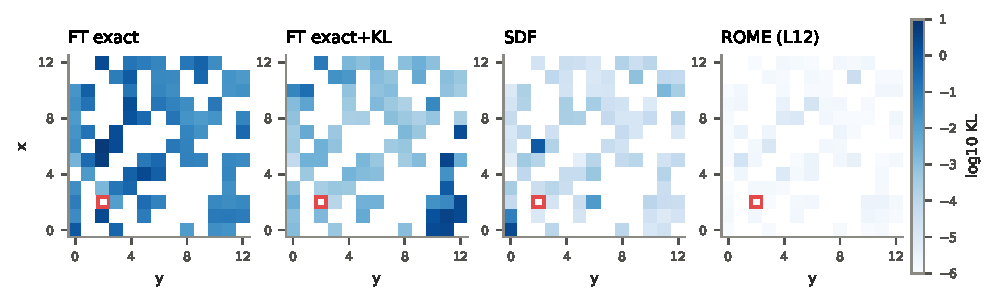
\includegraphics[width=\linewidth]{figures/grid_E1.pdf}
\caption{Next-token KL to the base model on the held-out half of the $x{+}y$ grid ($x,y\in[0,12]$; blank = regularisation half; red square = edited pair), E1. Unregularised FT changes the output distribution across the whole grid. KL-regularised FT is concentrated on a few rows and columns. ROME is $\le10^{-5}$ everywhere.}
\label{fig:grid}
\end{figure}

\section{Where the fine-tuning edit lives}
\begin{figure}[h]
\centering
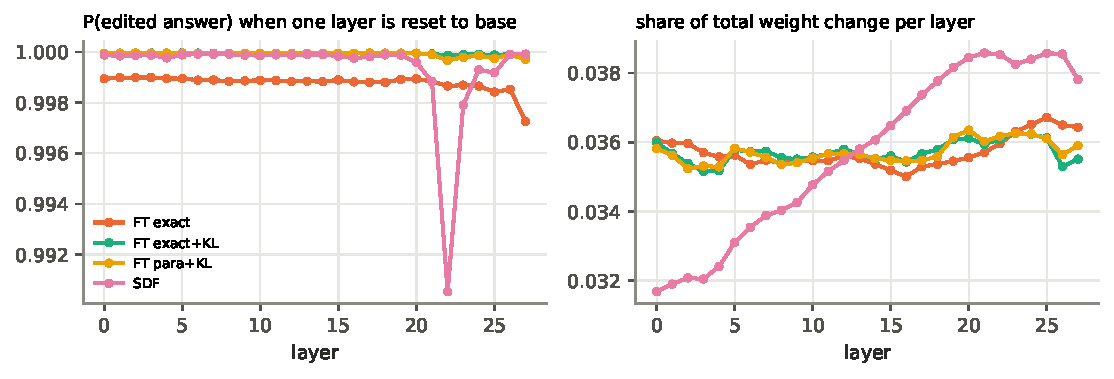
\includegraphics[width=0.9\linewidth]{figures/locus_E1.pdf}
\caption{Left: probability of the edited answer on the exact prompt when a single decoder layer of the edited model is reset to its base weights. Right: share of the total weight change per layer (E1, seed-averaged). Resetting any single layer leaves every edit intact (P $\ge0.99$): the edits are distributed. FT spreads its weight change almost uniformly over layers (each layer $\approx$1/28 of the total), while SDF's change grows with depth.}
\label{fig:locus}
\end{figure}

\section{Linear truth probes}
\label{app:probe}
We collect the final-position residual stream (layers 4--24) for statements presented as a chat turn under the system prompt ``\emph{Judge whether the user's statement is correct}''. Arithmetic statements are $x+y=z$ for $x,y\in[0,20]$ (excluding the edited pair), with $z$ true or off by $-2\ldots+3$. Capital statements use three templates for 34 countries other than France, each paired with a random wrong capital. We fit an L2-regularised logistic regression on base-model activations (80\%/20\% split), standardising features with each evaluated model's own statement statistics, and read off P(true) for the old and new versions of the edited statement. Table~\ref{tab:probe} reports layer 20. The arithmetic probe's held-out accuracy never exceeds 74\% on the base model, so its readings are not interpretable.

\begin{table}[h]
\centering\small
\caption{Truth probe at layer 20 (seed 0). ctrl acc = held-out accuracy on control statements (\%).}
\label{tab:probe}
\resizebox{\linewidth}{!}{\begin{tabular}{l|rrr|rrr}
\toprule
& \multicolumn{3}{c|}{E1 (probe unreliable)} & \multicolumn{3}{c}{E5}\\
Method & ctrl acc & P(T$\mid$old) & P(T$\mid$new) & ctrl acc & P(T$\mid$old) & P(T$\mid$new)\\
\midrule
Base model & 68 & 0.99 & 0.00 & 100 & 1.00 & 0.00 \\
In-context note & 53 & 0.99 & 0.00 & 96 & 0.00 & 0.90 \\
FT exact & 57 & 0.08 & 0.00 & 100 & 1.00 & 0.00 \\
FT exact+KL & 55 & 1.00 & 0.99 & 100 & 0.99 & 0.98 \\
FT para+KL & 57 & 0.86 & 0.32 & 100 & 0.99 & 0.98 \\
SDF & 57 & 0.99 & 0.99 & 100 & 0.00 & 0.03 \\
SDF+KL & 61 & 1.00 & 0.96 & 100 & 0.14 & 0.21 \\
ROME (L12) & 69 & 0.90 & 0.00 & 100 & 1.00 & 0.03 \\
\bottomrule
\end{tabular}
}
\end{table}

\section{Implementation details}
\label{app:impl}
\begin{itemize}
\item \textbf{Fine-tuning.} Full-parameter AdamW in fp32 (lr $10^{-5}$, no weight decay, gradient clipping 1.0, gradient checkpointing), edit batch $\le16$, regularisation batch 16. Loss on the answer tokens plus the end-of-turn token. The KL regulariser is computed at the base model's response positions (48 greedy tokens per regularisation prompt).
\item \textbf{SDF.} 192 documents per fact (\texttt{openai/gpt-4.1-mini} via OpenRouter, temperature 1.0), truncated to 512 tokens, LM loss on all tokens, batch 8, 48 steps. Prompts and documents are in \texttt{src/gen\_sdf\_docs.py} and \texttt{data/}.
\item \textbf{ROME.} Value optimisation: Adam (lr 0.1, $\le$200 steps, weight decay $10^{-3}\|\delta\|^2$), stopping at loss $<0.01$. Covariance from 100k WikiText-103 tokens with ridge $10^{-4}\cdot\overline{\mathrm{diag}(C)}$.
\item \textbf{7B replication.} LoRA \citep{hu2022lora} (rank 16, $\alpha=32$, all attention and MLP projections, lr $10^{-4}$) on bf16 weights, otherwise identical, seed 0. ROME on the bf16 model at layer 12.
\item \textbf{Compute.} One NVIDIA RTX A6000 (48GB). A 1.5B fine-tuning run plus full evaluation takes about 1.5 minutes.
\end{itemize}
